次に,セマンティックセグメンテーション分野におけるCNNについて説明する.
この分野における課題は,画像中に存在する物体を画素毎で精確に分類することである(\ref{fig:semantic_segmentation}).
\begin{figure}[ht]
  \centering
  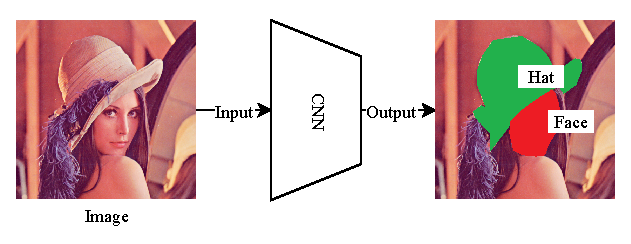
\includegraphics[width=16cm]{8_appendix/img/semantic_segmentation}
  \caption{Semantic Segmentation with CNN.}
  \label{fig:semantic_segmentation}
\end{figure}
自動運転や医療画像の分野において重要な技術であり、画像分類同様、セマンティックセグメンテーションにおいても CNNは多くの成果を収めている。
ここでは,その中でも代表的なモデルについて説明する.

\subsubsection{Fully Convolutional Networks(FCN)}
    Fully Convolutional Networks(FCN)とは,全ての層が畳み込み層で構成されたニューラルネットワークであり,最終的な出力が,物体の画素ごとのクラス確率となる.
    このネットワークでは,畳み込み層により特徴を抽出した後に,小さくなった画像サイズを出力サイズへ揃えるためのアップサンプリング用の畳み込み層(Deconvolution layer)が導入されている.
    損失には、ピクセル毎のクロスエントロピー誤差の合計を用いている。
    \begin{figure}[ht]
      \centering
      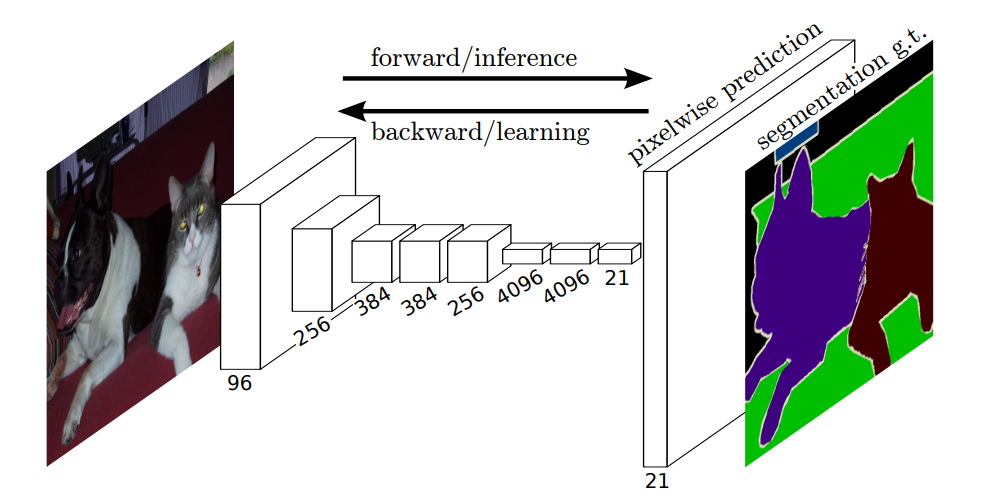
\includegraphics[width=12cm]{8_appendix/img/fcn}
      \caption{FCN architecture \cite{long2015fully}.}
    \end{figure}
    ダウンサンプリングされた特徴マップに対して単純に逆畳み込みを適用するだけでは、出力結果が粗くなってしまう。
    そのため、FCNではスキップ接続を用いて情報ロスが発生する前の情報をアップサンプリング層に入力する。
    \begin{figure}[ht]
      \centering
      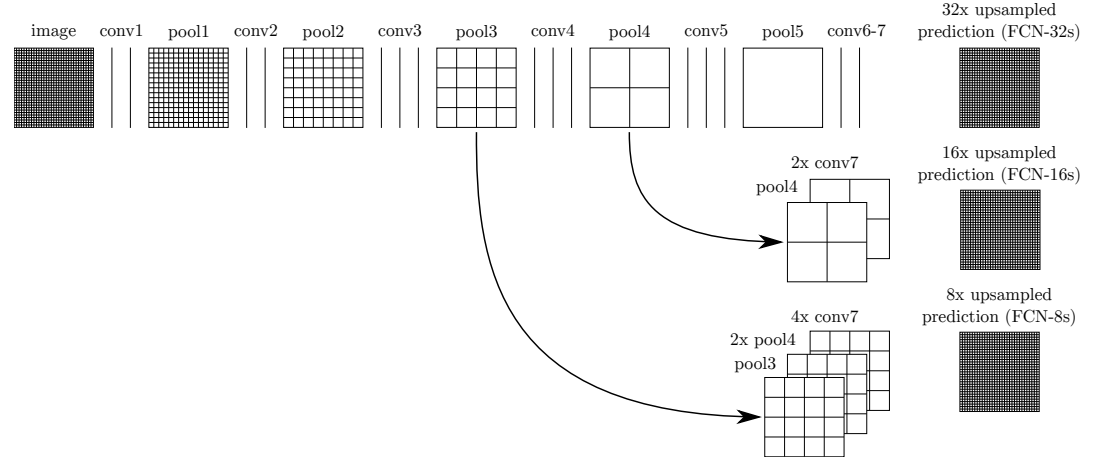
\includegraphics[width=12cm]{8_appendix/img/FCNskipconnect}
      \caption{FCN skipconnect architecture \cite{ronneberger2015u}.}
    \end{figure}
    
    このモデルの特徴は全結合層を使わない点であり、全結合層を畳み込み層に置き換えることで、出力を分類クラスではなく二次元マップに変更している。
    FCN以前はネットワーク内に全結合層が存在することにより、固定サイズの画像しか扱うことができなかったが、FCNでは全結合層が存在し
    ないため、あらゆるサイズの画像でセグメンテーションマップが生成できる。

\subsubsection{SegNet}
    SegNet\cite{badrinarayanan2017segnet}はエンコーダ(encoder)部分とデコーダ(decoder)部分で構成されるセマンティックセグメンテーションのためのネットワークである。
    FCNのスキップ接続ではプーリング前の特徴量をアップサンプリング層に入力していた。
    SegNetではエンコーダ部分のマックスプーリング層で採用した値の場所を記録し、デコーダ部分のアップサンプリング時にその位置情報を用いて特徴マップを拡大する。
    これによりデコード時に位置情報が保持され、FCNに比べてメモリ効率が向上した。

\subsubsection{U-Net}
    U-Net\cite{ronneberger2015u}は医療用のセマンティックセグメンテーションで大きな成果を残しているCNNアーキテクチャである.
    U-Netは、様々なスケールの特徴量を出力結果に利用するために,入力に近い層と出力に近い層の間を直接繋げる経路を導入したFCNである.
    \begin{figure}[ht]
      \centering
      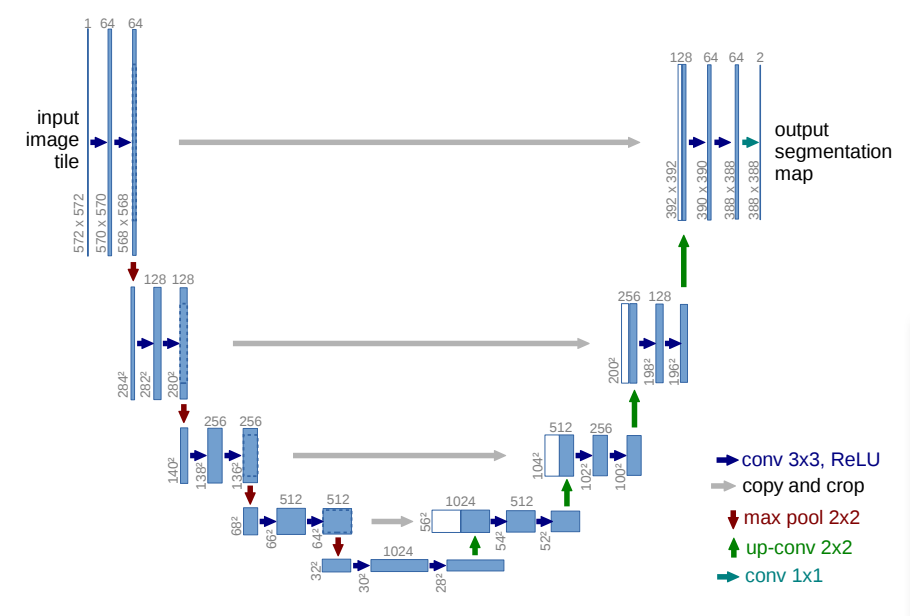
\includegraphics[width=12cm]{8_appendix/img/unet.png}
      \caption{U-Net architecture \cite{ronneberger2015u}.}
    \end{figure}

    入力側の特徴量を出力側へ反映する際、FCNやSegNetではチャンネルごとに加算を行っているが、U-Netは特徴量を連結することにより位置情報を保持している。
    これはResNetとDenseNetとの関係と同様である。

\subsubsection{PSPNet}
    PSPNet\cite{zhao2017pyramid}は、Pyramid Pooling Moduleを用いたEncoder–Decoder構造のSemantic Segmentationを行うモデルである。
    Pyramid Pooling Moduleでは、Encoderで抽出された特徴マップに対して、複数の解像度でmax-poolingをかけてそれぞれのスケールで捉えた特徴マップを得る。
    これによって、画像の大域的なコンテキストと小さな部分の情報の両方を拾うことができる。
    
    Pyramid Pooling Moduleの階層数や各階層での特徴マップのサイズは、入力される特徴マップのサイズに合わせて設計する。
    Pyramid Pooling Moduleの階層の数をNとすると、削減後の各特徴マップのチャンネル数は1/Nになる。
    
    論文の例では、階層的に4つの異なるカーネルサイズ(1×1, 2×2, 3×3, 6×6)でmax-poolingを行い、得られた複数スケールの特徴マップを1×1で畳み込んでチャンネル数を削減する。
    \begin{figure}[ht]
      \centering
      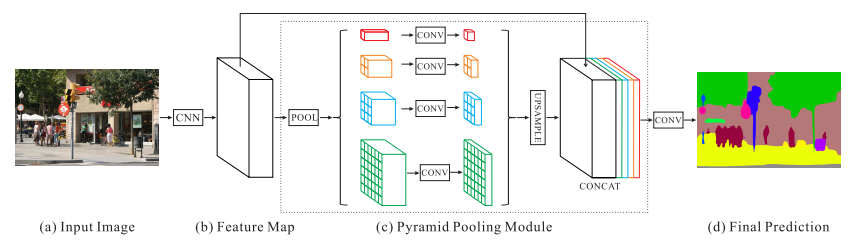
\includegraphics[width=15cm]{8_appendix/img/PyramidPoolingModule}
      \caption{Pyramid Pooling Module Architecture\cite{zhao2017pyramid}.}
      \label{fig:unet_architecture}
    \end{figure}
    
    そして、このチャンネル数を削減した特徴マップをバイリニア補間で元の特徴マップと同じサイズにアップサンプリングする。
    アップサンプリングしたこれらの特徴マップを元の特徴マップにチャンネルを追加する形で連結し、大域的なコンテキストと局所的な情報の両方を持った特徴マップとする。
    最終的に、この連結した特徴マップに対して1×1の畳み込みを行ってSemantic Segmentationの結果を得る。

\subsubsection{DeepLab}
    DeepLab\cite{chen2014semantic, chen2017deeplab}は、PSPNetのようにPyramid Pooling Moduleを用いたEncoder–Decoder構造のモデルである。
    DeepLabでは畳み込みにAtrous畳み込み(Dilated Convolution)を利用することで、パラメータの数や計算量を増やすことなく、フィルタの視野を効果的に拡大し、より大きなコンテキストを取り込むことができる。
    DeepLabではこの畳込みをArous spatial pyramid pooling (ASPP)と呼称している。
    他にも、DeepLabでは確率的グラフィカルモデルの手法を組み合わせることで、いくつかのピクセルが孤立して異なるクラスとして予測される問題を解消している。

